% !TeX spellcheck = de_DE
\documentclass{uebung_cs}
\usepackage{algo221}
\uebung{5}{}{}
\blattname{Übungen zu Woche 5: Randomisierte Algorithmen I}

%%%%%%%%%%%%%%%%%%%%%%%%%%%%%%%%%%%%%%%%%%%%%%%%%%%%%%%%%%%%%%%%%%%%%%%%%%%%
\begin{document}

Das Übungsblatt enthält alle empfohlenen Lernaktivitäten für die aktuelle Woche.

\begin{itemize}
\item \textbf{Heimarbeit bis Montag 17:00.}
    \begin{itemize}
    \item 
    Schau die Videos an und lies die Buchkapitel.
    \item Bearbeite die \emoji{seedling}-Aufgabe in \href{https://moodle.studiumdigitale.uni-frankfurt.de/moodle/course/view.php?id=2241}{Moodle}. (Feste Abgabefrist!)
    \item Lese den Aufgabentext aller Übungsaufgaben.
    \end{itemize}
\item \textbf{Heimarbeit.} Bearbeite die Übungsaufgaben soweit möglich. Probier zumindest alle mal!
\item \textbf{Dienstag/Donnerstag.}
\begin{itemize}
    \item \textbf{8:00--8:15.} Besprechung im Hörsaal.
    \item \textbf{8:15--9:15.} Bearbeite jetzt die Übungen, die du noch nicht lösen konntest. Sprich mit anderen Studis! Frag das Vorlesungsteam um Hilfe!
    \item \textbf{9:15--9:45.} Lösungsspaziergang zu den Aufgaben für heute.
\end{itemize}

\item \textbf{Heimarbeit bis Freitag, den 19.11., 17:00.} Gib deine Lösungen zu der \emoji{star}-Aufgabe von diesem Übungsblatt in \href{https://moodle.studiumdigitale.uni-frankfurt.de/moodle/course/view.php?id=2241}{Moodle} ab. (Feste Abgabefrist!)
\end{itemize}

\section*{Dienstag}

\begin{aufgabe}[Wahrscheinlichkeitsrechnung]\
	% Algorithms and Data Structures 2 - randomizedI.pdf
	Seien $E$ und $F$ zwei Ereignisse, für die $\Pr(E | F) = \Pr(E)$ und $\Pr(F | E) = P(F)$ gelten. Zeige, dass dann auch $\Pr(E \cap F) = \Pr(E) \cdot \Pr(F)$ gilt.
\end{aufgabe}

\begin{aufgabe}[Contention Resolution]\
	% Algorithms and Data Structures 2 - randomizedI.pdf
	\begin{enumerate}
		\item 
		Führe das \textit{contention resolution} Protokoll mit $4$ Prozessen aus. Benutze zwei Münzen, um die zufällige Auswahl zu simulieren. Wie viele Runden braucht man, bis alle Prozesse erfolgreich auf die Datenbank zugegriffen haben?
		\item Betrachte jetzt \textit{contention resolution} mit $n$ Prozessen und betrachte das Ereignis~$E$, dass mindestens einer der $n$ Prozesse in irgendeiner der $t$ Runden nicht auf die Datenbank zugreifen kann.
		Um die Wahrscheinlichkeit $\Pr(E)$ nach oben abzuschätzen wurde die \textit{union bound} angewendet. Sind die einzelnen Ereignisse hierbei disjunkt oder überschneiden sie sich?
	\end{enumerate}
\end{aufgabe}    

\begin{aufgabe}[Minimaler Schnitt]
	% Algorithms and Data Structures 2 - randomizedI.pdf
	Betrachte das \glqq kleine Graph\grqq{} Beispiel zum Kontraktionsalgorithmus, das wir in der Vorlesung behandelt haben. Löse die folgenden Aufgaben.
	\begin{center}
	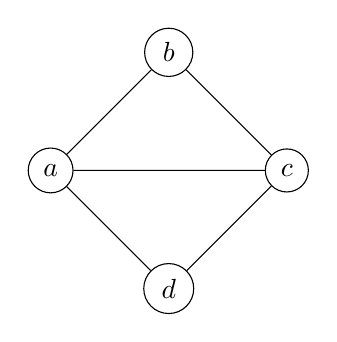
\begin{tikzpicture}
            \node[draw,circle] (a) at (0,0) {$a$};
            \node[draw,circle] (b) at (1.5,1.5) {$b$};
            \node[draw,circle] (d) at (1.5,-1.5) {$d$};
            \node[draw,circle] (c) at (3,0) {$c$};
            
            \draw  (a) -- (b)
                   (a) -- (c)
                   (a) -- (d)
                   (b) -- (c)
                   (c) -- (d);
        \end{tikzpicture}
	\end{center}
	\begin{enumerate}
		\item Zeige, dass es eine Sequenz von Kontraktionen gibt, die zu einem nicht minimalen Schnitt führen.
		\item Berechne die genaue Wahrscheinlichkeit, dass der Kontraktionsalgorithmus den minimalen Schnitt ausgibt.
	\end{enumerate}
\end{aufgabe}

\section*{Donnerstag}

\begin{aufgabe}[Schneller Kontraktionsalgorithmus]
	% Algorithms and Data Structures 2 - randomizedI.pdf
	Wie kann man den Kontraktionsalgorithmus für minimale Schnitte effizient implementieren? Beschreibe alle nötigen Datenstrukturen und Algorithmen, und analysiere die Laufzeit sowie den Platzverbrauch.
\end{aufgabe}

\begin{aufgabe}[Kontraktionsalgorithmus analysieren]
	% Algorithms and Data Structures 2 - randomizedI.pdf
	Betrachte die folgende Analyse der Erfolgswahrscheinlichkeit für den Kontraktionsalgorithmus. Die folgende Herleitung führt zum gewünschten Ergebnis:
	\begin{align}
	&\nonumber\Pr(E_{n-2} \cap \cdots \cap E_1) \\
	&\quad= \Pr(E_{n-3} \cap \cdots \cap E_1) \cdot \Pr(E_{n-2}|E_{n-3} \cap \cdots \cap E_1) \\
	&\quad= \Pr(E_1) \cdot \Pr(E_2|E_1) \cdots \Pr(E_{j+1} | E_j \cap \cdots \cap E_1) \cdots \Pr(E_{n-2} | E_{n-3} \cap \cdots \cap E_1) \\
	&\quad\ge \left(1 - \frac{2}{n} \right) \cdot \left(1 - \frac{2}{n-1} \right) \cdot \left(1 - \frac{2}{n-2} \right) \cdots \left(1 - \frac{2}{3} \right) \\
	&\quad= \left(\frac{n-2}{n}\right) \cdot \left(\frac{n-3}{n-1}\right) \cdot \left(\frac{n-4}{n-2}\right) \cdots \left(\frac{2}{4}\right) \cdot \left(\frac{1}{3}\right) \\
	&\quad= \left(\frac{2}{n(n-1)}\right) \geq \frac{2}{n^2}
	\end{align}
	Löse die folgenden Aufgaben.
	\begin{enumerate}
		\item Zeige (1) auf zwei Wege: Erstens, indem du die Formel für die bedingte Wahrscheinlichkeit benutzt, und zweitens, indem du interpretierst, was die linke und rechte Seite bedeuten.
		\item Zeige (2). \textit{Hinweis:} Benutze das Ergebnis aus Teilaufgabe a).
		\item Schätze jeden Faktor einzeln ab, um (3) zu zeigen. 
		\item Zeige (4).
		\item Zeige (5).
	\end{enumerate}
\end{aufgabe}

\begin{aufgabe}[Mehrheit]
	% Algorithms and Data Structures 2 - randomizedI.pdf
	Gegeben ist eine Sequenz $x_1,x_2,\dots,x_n$ von $n$ ganzen Zahlen. Die Sequenz hat das \textit{Mehrheitselement}~$t$, wenn die Zahl $t$ öfter als $\frac{n}{2}$-mal in der Sequenz vorkommt. Zum Beispiel hat die Sequenz $1,2,3,1,2,2,2$ das Mehrheitselement $2$, während die Sequenz $2,2,1,2,3,3$ kein Mehrheitselement hat.
	
	Hier ist ein randomisierter Algorithmus, um das Mehrheitselement zu finden: Ziehe eine uniform zufällige Zahl $x_i$ aus der Sequenz. Prüfe dann, ob diese Zahl öfter als $\frac{n}{2}$-mal in der Sequenz vorkommt. Wenn ja, ist es das Mehrheitselement. Wenn das nicht der Fall ist, gibt der Algorithmus aus, dass es kein Mehrheitselement gibt. Löse die folgenden Aufgaben.
	\begin{enumerate}
		\item Was ist die Laufzeit des Algorithmus?
		\item Kann der Algorithmus ein Mehrheitselement zurückgeben, wenn die Sequenz keins hat? Begründe deine Antwort.
		\item Kann der Algorithmus ausgeben, dass kein Mehrheitselement existiert, obwohl die Sequenz ein solches besitzt? Begründe deine Antwort.
		\item Bestimme die Wahrscheinlichkeit, dass der Algorithmus eine falsche Antwort liefert.
	\end{enumerate}
\end{aufgabe}

\section*{Sternaufgabe}

\begin{aufgabe}[\emoji{star}: Scheduling mit Independent Set]
	In Abschnitt 13.1 (\textbf{KT}) haben wir ein einfaches verteiltes Protokoll gesehen, um ein \textit{contention resolution} Problem zu lösen. Hier ist eine andere Möglichkeit, um \textit{contention resolution} mittels Randomisierung zu lösen, nämlich durch eine verteilte Konstruktion eines Independent Set.
	
	Wir haben ein System mit $n$ Aufgaben. Einige Paare von Aufgaben stehen im Konflikt, das heißt beide brauchen Zugang zu der gleichen Ressource. Das Ziel ist es, in einem gegebenen Zeitintervall ein möglichst großes Set $S$ ausführbarer Aufgaben zu finden, sodass keine zwei Aufgaben aus $S$ in einem Konflikt stehen. Das Set $S$ nennen wir \textit{konfliktfrei}.
	
	Man kann sich diesen Vorgang mit einem Graphen $G = (V,E)$ vorstellen. Dabei repräsentiert jeder Knoten $v \in V$ eine Aufgabe und eine Kante $e = (u,v)$ stellt einen Konflikt zwischen zwei Aufgaben $u$ und $v$ dar. Ist ein Set $S$ von Aufgaben konfliktfrei, bilden sie ein Independent Set in $G$. Da man das allgemeine Independent Set Problem auf dieses Problem reduzieren kann, ist es schwierig, ein maximales und konfliktfreies Set $S$ für einen beliebigen Konfliktgraphen $G$ zu finden. Dennoch können wir uns eine Heuristik anschauen, die ein vernünftig großes und konfliktfreies Set findet. Dafür überlegen wir uns eine einfache dezentralisierte Methode: Jede Aufgabe kommuniziert nur mit einer kleinen Anzahl anderer Aufgaben und entscheidet dann, ob sie in das Set $S$ gehört oder nicht.
	
	Wir nehmen an, dass jeder Knoten genau $d$ Nachbarn in $G$ hat. Das heißt, jede Aufgabe hat einen Konflikt zu genau $d$ anderen Aufgaben.
	Schaue dir nun das folgende Verfahren an:
	\begin{quote}
		Jede Aufgabe $P_i$ wählt unabhängig einen zufälligen Wert $x_i$. Dabei nimmt $x_i$ mit einer Wahrscheinlichkeit von $\frac{1}{2}$ den Wert $0$ und mit einer Wahrscheinlichkeit von $\frac{1}{2}$ den Wert $1$ an. Die Aufgabe gehört genau dann in das Set $S$, wenn sie $x_i = 1$ gewählt hat und jede Aufgabe, mit der sie im Konflikt steht, den Wert $0$ gewählt hat.
	\end{quote}
	Zeige, dass das dadurch entstandene Set $S$ konfliktfrei ist. Gib außerdem eine Formel für die erwartete Größe von $S$ in Abhängigkeit  der Anzahl an Aufgaben $n$ und der Anzahl an Konflikten $d$ an.
\end{aufgabe}

\end{document}
